\chapter{分治算法之第 K 极值}
\begin{introduction}
	\item 问题引入
	\item 分治思路
	\item 复杂度分析
	\item 优化
	\item 其他值得关注的点
	\item 分治思路
	
\end{introduction}
\section{问题引入}
给定一个长度为 $n$的序列 $N$,求整个序列中第 $k$小的数。
\section{分治思路}
称这个问题为$\text { question }(N, k)$,模仿快速排序的做法,在序列中随机选择一个数作为中间标记tag后将
小于tag数放到tag左边,其余数放到tag右边。
\begin{figure}[h]
	\begin{minipage}[t]{1\linewidth}
		\centering
		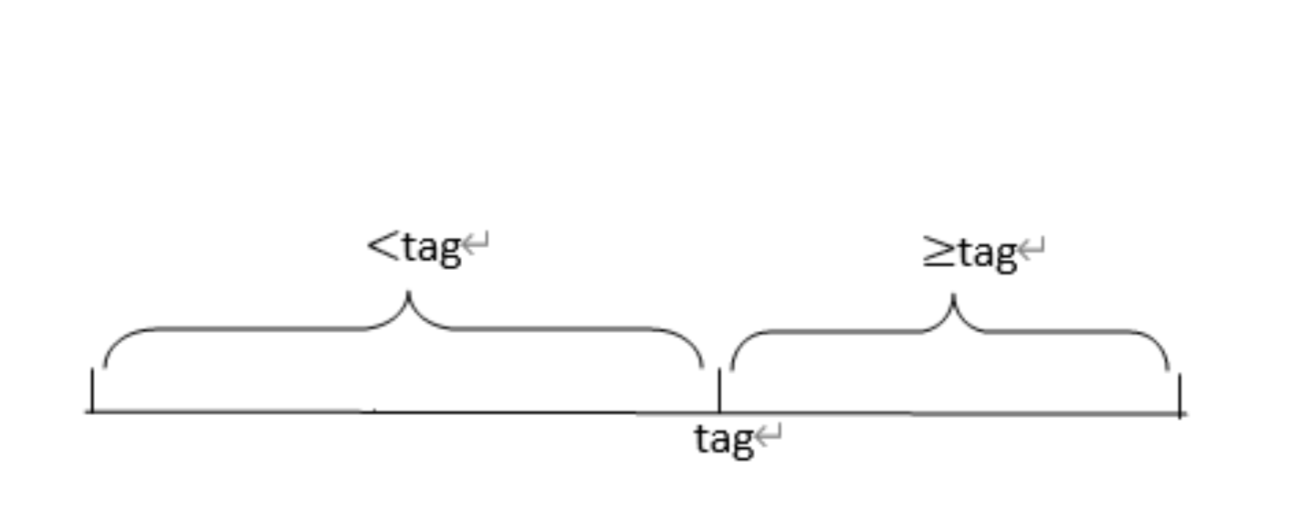
\includegraphics[width=10cm,height=3.5cm]{image/kth1.png}
		\caption{模仿快速排序}
	\end{minipage}
\end{figure}
这样我们得到了两个小一点的序列。为了后文的叙述方便,我们称在  t a g  左 侧的序列为  $N_{l}$,  长度为  $\left|N_{l}\right|$,  在$ \operatorname{tag}$ 右侧的序列为 $N_{r}$,  长度为$  \left|N_{r}\right|$ 。
到这一步,我们将问题拆解为如下三种情况:
$$
\text {question}(N, k)=\left\{\begin{aligned}
\text {question}\left(N_{l}, k\right) ,&\left|N_{l}\right|>=k \\
\text {tag} ,&\left|N_{l}\right|=k-1 \\
\text {question}\left(N_{r}, k-\left|N_{l}\right|-1\right) ,&\left|N_{l}\right|<k-1
\end{aligned}\right.
$$
按照上述方法不断递归下去,直到中间某一步达成 $ \left|N_{l}\right|=k-1$  的条件时, 就得到想要的结果了。
\section{复杂度分析}
因为算法中每一步的 tag都是随机取的,所以我们在分析复杂度时不仅要 考虑理想情况,也要考虑最坏情况。
最佳情况  \quad  每一次的  t a g  都恰好为序列的中间值,即每次操作都将问题规 模缩小为原来的一半。于是由经典的分治算法复杂度计算我们可以得到:
$$T(n)=T\left(\frac{n}{2}\right)+n$$
由主定理可以得到此时的时间复杂度
$$T(n) \in O(n)$$

最坏情况 每一次tag都恰好为序列的最大值或者最小值,即每次操作都 只能将问题规模减 1。于是我们可以的得到:
$$
T(n)=1+2+3+\cdots+(n-1)+n
$$
即
$$
T(n)=\frac{n(n+1)}{2}
$$
所以最坏情况的时间复杂度
$$
T(n) \in O\left(n^{2}\right)
$$
中间情况  \quad  我们虽然很难保证每次  t a g  的选取都恰好选中序列的中间值,但
如果我们能保证每次选取的  t a g  都在某个区间范围内,这种中间情况会比 最坏情况好很多。
比如,假如我们能够保证每次操作得到的  
$$\left|N_{l}\right|  $$
都满足式:

$$\frac{1}{4}|N| \leq\left|N_{l}\right| \leq \frac{3}{4}|N|$$

